\documentclass{standalone}
\usepackage{tikz}
\usetikzlibrary{patterns, positioning}
\usepackage[sfdefault]{ClearSans} %% option 'sfdefault' activates Clear Sans as the default text font
\usepackage[T1]{fontenc}

\begin{document}
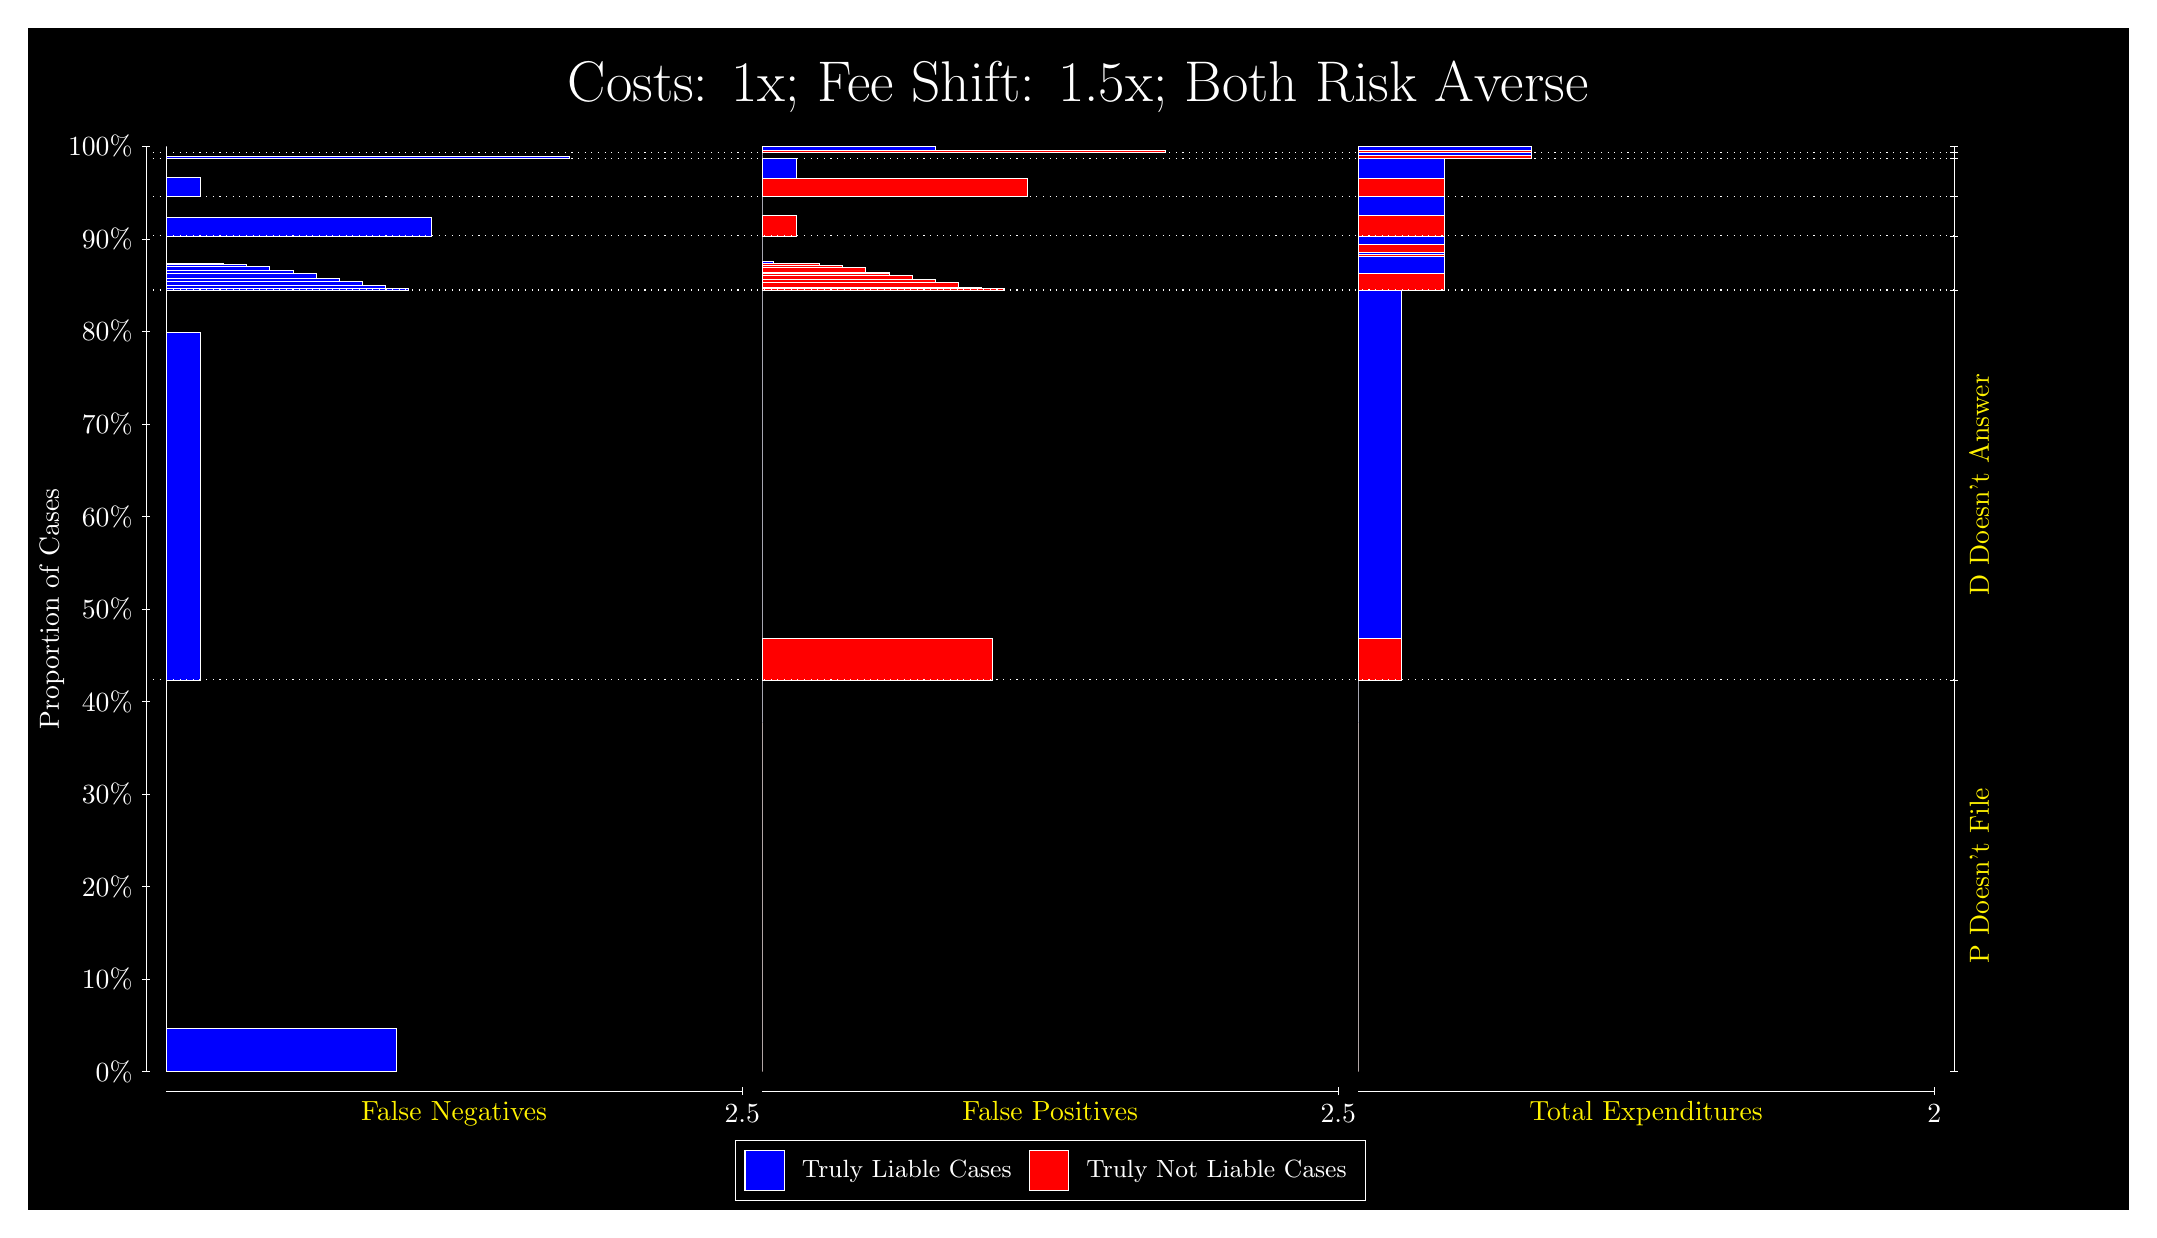
\begin{tikzpicture}
\draw[fill=black] (0,0) rectangle (26.667,15);
\draw[text=white] (0,13.5) rectangle (26.667,15) node[midway] {\huge Costs: 1x; Fee Shift: 1.5x; Both Risk Averse};
\draw[white, very thin] (1.5,1.75) -- (1.5,13.5);
\node[rotate=90, text=white, anchor=center] at (0.3, 7.625) {Proportion of Cases};
\draw[white, very thin] (1.45,1.75) -- (1.55,1.75);
\node[text=white, anchor=east] at (1.45, 1.75) {0\%};
\draw[white, very thin] (1.45,2.925) -- (1.55,2.925);
\node[text=white, anchor=east] at (1.45, 2.925) {10\%};
\draw[white, very thin] (1.45,4.1) -- (1.55,4.1);
\node[text=white, anchor=east] at (1.45, 4.1) {20\%};
\draw[white, very thin] (1.45,5.275) -- (1.55,5.275);
\node[text=white, anchor=east] at (1.45, 5.275) {30\%};
\draw[white, very thin] (1.45,6.45) -- (1.55,6.45);
\node[text=white, anchor=east] at (1.45, 6.45) {40\%};
\draw[white, very thin] (1.45,7.625) -- (1.55,7.625);
\node[text=white, anchor=east] at (1.45, 7.625) {50\%};
\draw[white, very thin] (1.45,8.8) -- (1.55,8.8);
\node[text=white, anchor=east] at (1.45, 8.8) {60\%};
\draw[white, very thin] (1.45,9.975) -- (1.55,9.975);
\node[text=white, anchor=east] at (1.45, 9.975) {70\%};
\draw[white, very thin] (1.45,11.15) -- (1.55,11.15);
\node[text=white, anchor=east] at (1.45, 11.15) {80\%};
\draw[white, very thin] (1.45,12.325) -- (1.55,12.325);
\node[text=white, anchor=east] at (1.45, 12.325) {90\%};
\draw[white, very thin] (1.45,13.5) -- (1.55,13.5);
\node[text=white, anchor=east] at (1.45, 13.5) {100\%};

\draw[white, very thin] (24.457,1.75) -- (24.457,13.5);
\draw[white, very thin] (24.407,1.75) -- (24.507,1.75);
\node[anchor=west] at (24.407, 1.75) {};
\draw[white, very thin] (24.407,6.7245) -- (24.507,6.7245);
\node[anchor=west] at (24.407, 6.7245) {};
\draw[white, very thin] (24.407,11.675) -- (24.507,11.675);
\node[anchor=west] at (24.407, 11.675) {};
\draw[white, very thin] (24.407,12.363) -- (24.507,12.363);
\node[anchor=west] at (24.407, 12.363) {};
\draw[white, very thin] (24.407,12.861) -- (24.507,12.861);
\node[anchor=west] at (24.407, 12.861) {};
\draw[white, very thin] (24.407,13.342) -- (24.507,13.342);
\node[anchor=west] at (24.407, 13.342) {};
\draw[white, very thin] (24.407,13.42) -- (24.507,13.42);
\node[anchor=west] at (24.407, 13.42) {};
\draw[white, very thin] (24.407,13.5) -- (24.507,13.5);
\node[anchor=west] at (24.407, 13.5) {};

\draw[white, very thin, fill=blue] (1.75,1.75) rectangle (4.6775,2.2931);
\draw[white, very thin, fill=red] (1.75,2.2931) rectangle (1.75,6.7245);
\draw[white, very thin, fill=blue] (1.75,6.7245) rectangle (2.1891,11.144);
\draw[white, very thin, fill=red] (1.75,11.144) rectangle (1.75,11.675);
\draw[white, very thin, fill=blue] (1.75,11.675) rectangle (4.8239,11.702);
\draw[white, very thin, fill=blue] (1.75,11.702) rectangle (4.5312,11.73);
\draw[white, very thin, fill=blue] (1.75,11.73) rectangle (4.2384,11.791);
\draw[white, very thin, fill=blue] (1.75,11.791) rectangle (3.9457,11.828);
\draw[white, very thin, fill=blue] (1.75,11.828) rectangle (3.6529,11.883);
\draw[white, very thin, fill=blue] (1.75,11.883) rectangle (3.3602,11.921);
\draw[white, very thin, fill=blue] (1.75,11.921) rectangle (3.0674,11.979);
\draw[white, very thin, fill=blue] (1.75,11.979) rectangle (2.7746,12);
\draw[white, very thin, fill=blue] (1.75,12) rectangle (2.4819,12.019);
\draw[white, very thin, fill=red] (1.75,12.019) rectangle (1.75,12.363);
\draw[white, very thin, fill=blue] (1.75,12.363) rectangle (5.1167,12.602);
\draw[white, very thin, fill=red] (1.75,12.602) rectangle (1.75,12.861);
\draw[white, very thin, fill=blue] (1.75,12.861) rectangle (2.1891,13.111);
\draw[white, very thin, fill=red] (1.75,13.111) rectangle (1.75,13.342);
\draw[white, very thin, fill=blue] (1.75,13.342) rectangle (6.8732,13.377);
\draw[white, very thin, fill=red] (1.75,13.377) rectangle (1.75,13.42);
\draw[white, very thin, fill=red] (1.75,13.42) rectangle (1.75,13.456);
\draw[white, very thin, fill=blue] (1.75,13.456) rectangle (1.75,13.5);
\draw[white, very thin, fill=red] (9.3189,1.75) rectangle (9.3189,6.1814);
\draw[white, very thin, fill=blue] (9.3189,6.1814) rectangle (9.3189,6.7245);
\draw[white, very thin, fill=red] (9.3189,6.7245) rectangle (12.246,7.2559);
\draw[white, very thin, fill=blue] (9.3189,7.2559) rectangle (9.3189,11.675);
\draw[white, very thin, fill=red] (9.3189,11.675) rectangle (12.393,11.692);
\draw[white, very thin, fill=red] (9.3189,11.692) rectangle (12.1,11.713);
\draw[white, very thin, fill=red] (9.3189,11.713) rectangle (11.807,11.77);
\draw[white, very thin, fill=red] (9.3189,11.77) rectangle (11.515,11.808);
\draw[white, very thin, fill=red] (9.3189,11.808) rectangle (11.222,11.863);
\draw[white, very thin, fill=red] (9.3189,11.863) rectangle (10.929,11.885);
\draw[white, very thin, fill=red] (9.3189,11.885) rectangle (10.929,11.901);
\draw[white, very thin, fill=red] (9.3189,11.901) rectangle (10.636,11.962);
\draw[white, very thin, fill=red] (9.3189,11.962) rectangle (10.344,11.989);
\draw[white, very thin, fill=red] (9.3189,11.989) rectangle (10.051,12.02);
\draw[white, very thin, fill=blue] (9.3189,12.02) rectangle (9.4652,12.039);
\draw[white, very thin, fill=blue] (9.3189,12.039) rectangle (9.3189,12.363);
\draw[white, very thin, fill=red] (9.3189,12.363) rectangle (9.758,12.622);
\draw[white, very thin, fill=blue] (9.3189,12.622) rectangle (9.3189,12.861);
\draw[white, very thin, fill=red] (9.3189,12.861) rectangle (12.686,13.091);
\draw[white, very thin, fill=blue] (9.3189,13.091) rectangle (9.758,13.342);
\draw[white, very thin, fill=red] (9.3189,13.342) rectangle (9.3189,13.385);
\draw[white, very thin, fill=blue] (9.3189,13.385) rectangle (9.3189,13.42);
\draw[white, very thin, fill=red] (9.3189,13.42) rectangle (14.442,13.456);
\draw[white, very thin, fill=blue] (9.3189,13.456) rectangle (11.515,13.5);
\draw[white, very thin, fill=red] (16.888,1.75) rectangle (16.888,6.1814);
\draw[white, very thin, fill=blue] (16.888,6.1814) rectangle (16.888,6.7245);
\draw[white, very thin, fill=red] (16.888,6.7245) rectangle (17.437,7.2559);
\draw[white, very thin, fill=blue] (16.888,7.2559) rectangle (17.437,11.675);
\draw[white, very thin, fill=red] (16.888,11.675) rectangle (17.986,11.885);
\draw[white, very thin, fill=blue] (16.888,11.885) rectangle (17.986,12.098);
\draw[white, very thin, fill=red] (16.888,12.098) rectangle (17.986,12.128);
\draw[white, very thin, fill=blue] (16.888,12.128) rectangle (17.986,12.155);
\draw[white, very thin, fill=red] (16.888,12.155) rectangle (17.986,12.259);
\draw[white, very thin, fill=blue] (16.888,12.259) rectangle (17.986,12.363);
\draw[white, very thin, fill=red] (16.888,12.363) rectangle (17.986,12.622);
\draw[white, very thin, fill=blue] (16.888,12.622) rectangle (17.986,12.861);
\draw[white, very thin, fill=red] (16.888,12.861) rectangle (17.986,13.091);
\draw[white, very thin, fill=blue] (16.888,13.091) rectangle (17.986,13.342);
\draw[white, very thin, fill=red] (16.888,13.342) rectangle (19.083,13.385);
\draw[white, very thin, fill=blue] (16.888,13.385) rectangle (19.083,13.42);
\draw[white, very thin, fill=red] (16.888,13.42) rectangle (19.083,13.456);
\draw[white, very thin, fill=blue] (16.888,13.456) rectangle (19.083,13.5);
\draw[white, dotted] (1.5,6.7245) -- (24.457,6.7245);
\draw[white, dotted] (1.5,11.675) -- (24.457,11.675);
\draw[white, dotted] (1.5,12.363) -- (24.457,12.363);
\draw[white, dotted] (1.5,12.861) -- (24.457,12.861);
\draw[white, dotted] (1.5,13.342) -- (24.457,13.342);
\draw[white, dotted] (1.5,13.42) -- (24.457,13.42);
\draw[white, very thin] (1.75,1.5) -- (9.0689,1.5);
\node[text=yellow, anchor=north] at (5.4094, 1.5) {False Negatives};
\draw[white, very thin] (9.0689,1.45) -- (9.0689,1.55);
\node[text=white, anchor=north] at (9.0689, 1.45) {2.5};

\draw[white, very thin] (9.3189,1.5) -- (16.638,1.5);
\node[text=yellow, anchor=north] at (12.978, 1.5) {False Positives};
\draw[white, very thin] (16.638,1.45) -- (16.638,1.55);
\node[text=white, anchor=north] at (16.638, 1.45) {2.5};

\draw[white, very thin] (16.888,1.5) -- (24.207,1.5);
\node[text=yellow, anchor=north] at (20.547, 1.5) {Total Expenditures};
\draw[white, very thin] (24.207,1.45) -- (24.207,1.55);
\node[text=white, anchor=north] at (24.207, 1.45) {2};

\node[text=yellow, centered, rotate=90] at (24.777, 4.2373) {P Doesn't File};
\node[text=yellow, centered, rotate=90] at (24.777, 9.2) {D Doesn't Answer};






\draw (12.978300999999998,1.5) node[draw=none] (baseCoordinate) {};
\begin{scope}[align=center]
        \matrix[scale=0.5, draw=white, below=0.5cm of baseCoordinate, nodes={draw}, column sep=0.1cm]{
            \node[rectangle, draw, minimum width=0.5cm, minimum height=0.5cm, fill=blue] {}; &
            \node[draw=none, font=\small, text=white] (B) {Truly Liable Cases}; &
            \node[rectangle, draw, minimum width=0.5cm, minimum height=0.5cm, fill=red] {}; &
            \node[draw=none, font=\small, text=white] (B) {Truly Not Liable Cases}; \\
            };
\end{scope}

\end{tikzpicture}
\end{document}